\documentclass[tikz,border=10pt]{standalone}
\usepackage{tikz}
\usetikzlibrary{positioning}
\usetikzlibrary{shapes.geometric}% tikz node 形状的库
\usetikzlibrary{patterns}
\usepackage{tikz-feynman}
\begin{document}

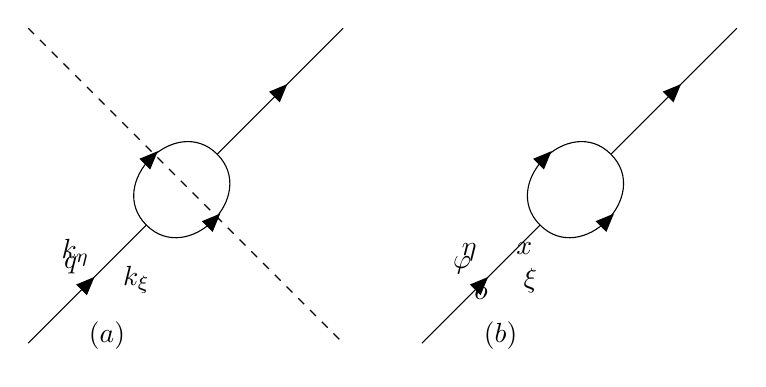
\begin{tikzpicture}[scale=.5]
	\begin{feynman}
		%% fig a
		\vertex (a1) at (0,0);
		\node at (2,.2) {$(a)$};
		\vertex[above right = 4 and 4 of a1] (a2);
		\vertex[above right = 4 and 0 of a1] (a3);
		\vertex[above right = 0 and 4 of a1] (a4);
		\vertex[above right = 1.5 and 1.5 of a1] (a5);
		\vertex[above right = 2.4 and 2.4 of a1] (a6);
		\node at (1.2,2.3) {$k_\eta$};
		\node at (2.75,1.6) {$k_\xi$};
		% 对各个顶点连线
		\diagram*{
		(a3)--[scalar](a4);
		(a1) --[fermion,edge label = \(q\)] (a5)--[fermion,half left,looseness=1.5] (a6)--[fermion](a2);
		(a5)--[fermion,half right,looseness=1.5](a6);
		};
	\end{feynman}
	\begin{feynman}[xshift=10cm]
		%% fig a
		\vertex (a1) at (0,0);
		\node at (2,.2) {$(b)$};
		\vertex[above right = 4 and 4 of a1] (a2);
		\vertex[above right = 1.5 and 1.5 of a1] (a5);
		\node at (1.5,1.25) {$o$};
		\vertex[above right = 2.4 and 2.4 of a1] (a6);
		\node at (2.6,2.4) {$x$};
		\node at (1.2,2.3) {$\eta$};
		\node at (2.75,1.6) {$\xi$};
		% 对各个顶点连线
		\diagram*{
		(a1) --[fermion,edge label = \(\varphi\)] (a5)--[fermion,half left,looseness=1.5] (a6)--[fermion](a2);
		(a5)--[fermion,half right,looseness=1.5](a6);
		};
	\end{feynman}
\end{tikzpicture}

\end{document}
